\section{进阶功能的使用}
\subsection{参考文献和引用}
没有人希望看到自己辛苦撰写的毕业论文被判定为抄袭,而抄袭与合理的引用的差别仅仅在于作者有没有在文中明确的标注自己所引用文献的出处。而\TeX 作为严谨的科学论文排版体系,对于文献引用进行了完善的设计。用户需要学习如何通过合理的手段取得这些文献,并且恰当地引用他们来佐证自己的观点。
相信通过这样的学习,每个用户都能严肃而认真地对待论文引用的问题。
\subsubsection{来源——高效的文献管理软件}

随着网络和电子技术的发展,图书馆的信息收集和服务等也越来越多的实现了电子化和网络化。各种类型的图书馆纷纷建立自己的电子信息服务系统来追赶这一发展趋势。与此同时,由于信息传播的路径越来越多和越来越便捷,文献服务的时效性也变得非常突出,用户需要其机构图书馆能够提供及时的文献动态服务。同时,众多的学校和研究机构图书馆开始购买国内外各种电子资源数据库,面对海量的研究信息,往往让缺少文献信息收集和管理的研究者却步,这在一定程度上也影响了学校购买的昂贵的电子资源的使用效率和最终的研究成果产出。
面对海量文献信息的电子化,信息过滤和管理变得极其重要,为了提高研究者对电子资源的使用效率,为了帮助研究者有效管理和利用这些电子文献,文献管理类软件应运而生。作为中国大陆和台湾等地高校和研究院所非常受欢迎的文献管理软件NoteExpress的开发商——北京爱琴海乐之技术有限公司,我们为众多研究人员提供了专业的文献信息管理解决方案。NoteExpress已经成为中国文献管理软件市场上的第一品牌,拥有绝对领先的软件性能和市场优势。NoteExpress 围绕科学研究最核心的文献信息,为用户提供了信息导入、过滤、全文下载,以及众多的管理功能,可以大大提高研究者的文献管理和研究效率。

这是一个很好用的软件,学生版本的最低售价是198元,但是我们学校买了他的集团版本,所以只要用户拥有武汉理工大学的注册在籍学生身份就能完全免费的使用。这也是任何一个决心搞科研必备的同学素质:既然选择了科研事业,就要有向全人类要吃要喝的决心。
\subsubsection{实现——Bib\TeX 系统}
Bib\TeX 是\LaTeX 独有的文献管理系统,通过Bib\TeX 我们可以很方便的完成文献的引用。比如说现在我们要引用一篇题为《LaTeX与方正书版排版数学论文探讨》的文章,传统的Bib\TeX 做法是去网络上手动的把他的信息给扒下来,俗称“人肉论文引用机”。但这样做是我们后面工作的基础,因为巧妇难为无米之炊我们需要引用文章的基本信息这样才能够在合适的位置显示他们。
在Bib\TeX 中,我们需要的基本信息有题名,作者,期刊名,出版年份,甚至出现的页数等等信息
得到这些信息之后把他们写到Bib\TeX 文件里,例子里面的信息应该呈现出这样的样式。
\begin{lstlisting}[language=TeX]
@article{
王勇姚萍-197,
   Author = { 王勇 and 姚萍 and 王岚 and 庞立},
   Title = {LaTeX 与方正书版排版数学论文探讨},
   Journal = { 中国科技期刊研究} ,
   Year = {2012} }

\end{lstlisting}
拥有这样的信息之后就可以在文章中出现他们引用的地方用\textbackslash cite命令完成引用,并且在文章最后的引用文献中按照规范(GBT7714-2005N)列出他们。假设我们引用了《LaTeX与方正书版排版数学论文探讨》中的内容“LaTeX不知道要比方正高明到哪里去了!"\cite{王勇姚萍-197},那么以上就应该是你所见到文章中的样式。这里再举一个例子,关于字体的设计我们有很多话要说。\cite{吴昉张页-198}
\subsubsection{结合——管理自己的文献}
首先用户需要到NoteExpress网站上自行下载武汉理工大学专版的软件,安装完毕后打开软件。
\begin{figure}[htbp]
\centering
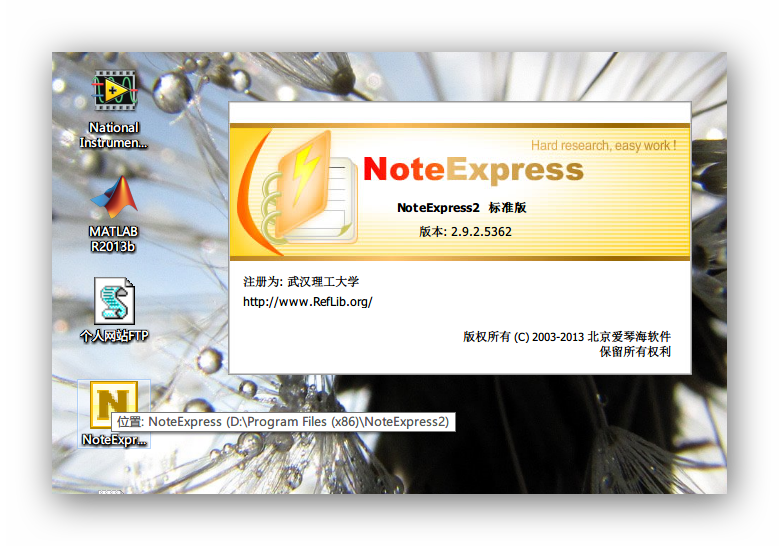
\includegraphics[width=7cm]{figure/1}
\caption{启动软件}
\label{fig:1}
\end{figure} \\

打开软件之后选择检索菜单里面的在线检索,根据自己的文档类型选择合适的数据库。
\begin{figure}[htb]
\centering
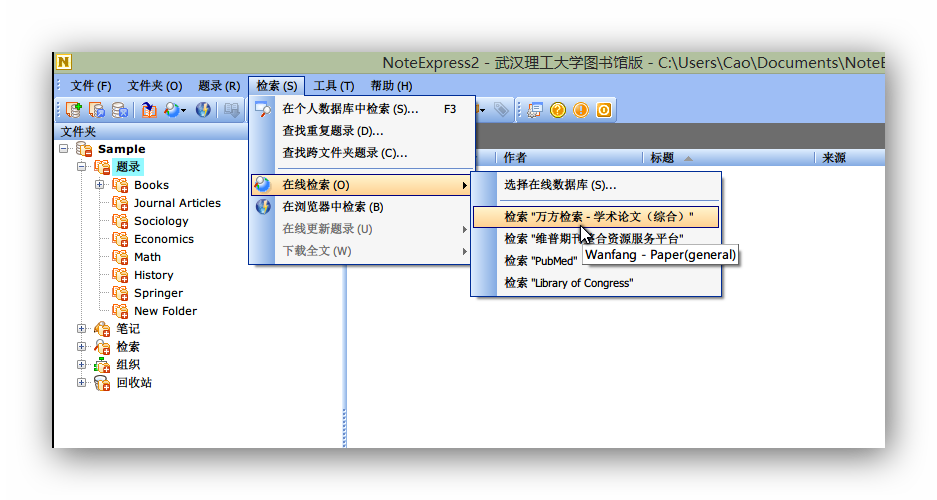
\includegraphics[width=7cm]{figure/2}
\caption{检索文档}
\label{fig:2}
\end{figure} \\

对于非校园网还需要设置一下代理来完成对于校内资源的访问。
\begin{figure}[htbp]
\centering
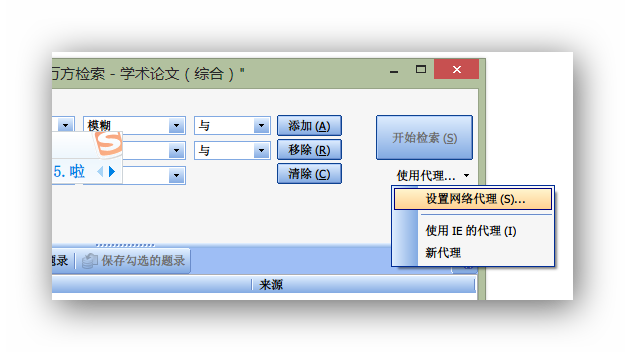
\includegraphics[width=7cm]{figure/3}
\end{figure}\\

设置参数,图中学号应为饭卡号,在此更正。
\begin{figure}[htbp]
\centering
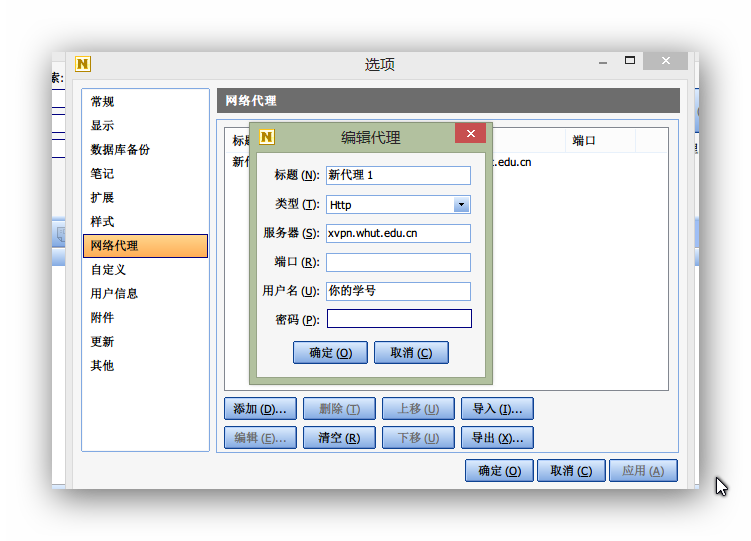
\includegraphics[width=7cm]{figure/4}
\end{figure}\\

找到所需要的参考文献,并放置到合适的位置如图书,期刊等。
\begin{figure}[htbp]
\centering
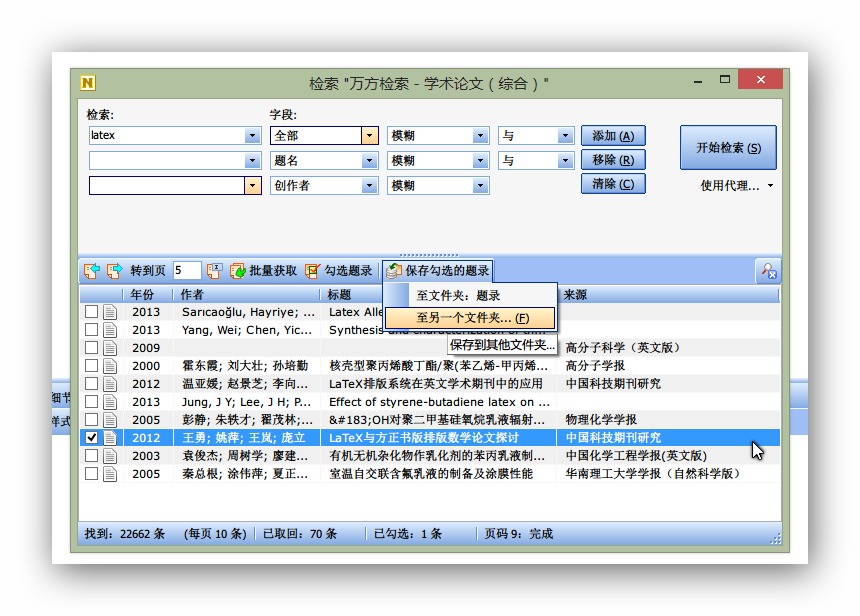
\includegraphics[width=7cm]{figure/5}
\end{figure}\\

此时就可以在主程序窗体中看到所引用的文献信息了,
\begin{figure}[htbp]
\centering
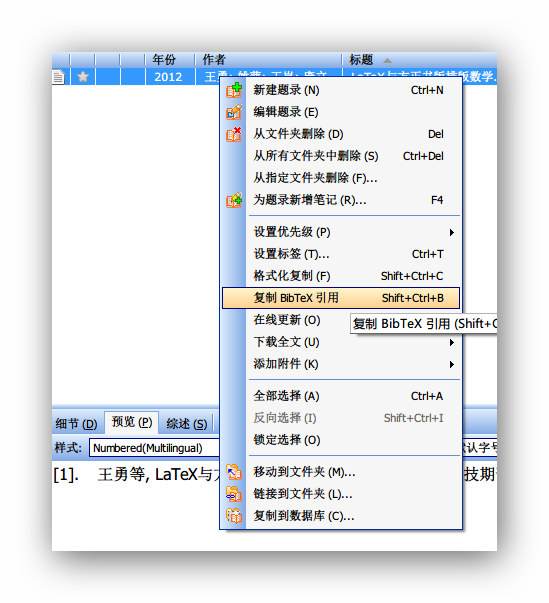
\includegraphics[width=7cm]{figure/7}
\end{figure}
引用时:右键单击该条目,复制出Bib\TeX 引用的信息,粘贴到所引用位置即可。
在本模板的figure文件夹下有后续步骤的图片示意。用户可以对照NoteExpress使用手册,以及这几个示意图完成设置使用的过程。

\subsection{在线编辑和共享}
在线编辑为用户提供了脱离本地环境的编译体验,也方便了文档进行共享和传递。通常来说,用户最终呈现的毕业论文应该是经过编译之后的pdf文件。这个文件满足一般设备的需求,可以在个人电脑,平板电脑,电子书阅读器等设备上获得优良的观感体验。更重要的是可以按照文档所见的样子通过打印机获得质量上乘的纸质副本,满足纸质论文的一切需求。\\

但是在\LaTeX 的使用过程中,我们可能会面临多人撰写同一个论文的情况,比如第一作者完成前言和导论的内容,第二作者完善第一章,第三作者帮助进行图标的处理。这样就需要我们传递原始的\TeX 原档来进行合作,这样做缺点非常明显:每个人的处理步骤不同步导致文档在整体上的形式不符合要求。要解决这个问题,就需要诸如本模板之类的模板文件的帮助。用户在请求共享和协作的时候,应该给所有协作者分发模板的全部内容。同时协作者应该帮助完成body里的内容,而不允许修改thesis.tex这个控制文件。用户在收到协作者的body文件之后再用include的命令把他们写入到总体框架中去。这种方法是国际期刊通行的处理方法,用户可以借鉴使用。\\

除此之外,我们还可以利用GITHUB来帮助我们进行论文的协作写作,每个独立的作者
应该拥有自己的协作者账号。在对于的论文项目下,采用merge的形式进行文档的增补和修订,这样做的好处在于GITHUB拥有完善的修订记录,可以很方便的对于不同的修订内容进行采纳或拒绝。这也给了用户给大的自由度,他们可以对于控制文件的结构提出修改,从而使论文的样式和结构更加完美。